\documentclass[aspectratio=169,10pt]{beamer}

\usepackage[T1]{fontenc}
\usepackage{lmodern}
\usepackage{graphicx}
\usepackage{tikz}
\usetikzlibrary{arrows.meta,positioning}

\graphicspath{{figs/}}

\definecolor{HopkinsBlue}{HTML}{002D72}
\definecolor{SpiritBlue}{HTML}{68ACE5}
\definecolor{DeepBlue}{HTML}{001B44}
\definecolor{PaleBlue}{HTML}{EAF4FB}
\definecolor{Muted}{HTML}{526777}

\setbeamercolor{normal text}{fg=DeepBlue,bg=white}
\setbeamercolor{structure}{fg=HopkinsBlue}
\setbeamercolor{frametitle}{fg=white,bg=HopkinsBlue}
\setbeamercolor{title}{fg=HopkinsBlue}
\setbeamercolor{subtitle}{fg=Muted}
\setbeamercolor{block title}{fg=white,bg=HopkinsBlue}
\setbeamercolor{block body}{fg=DeepBlue,bg=PaleBlue}
\setbeamercolor{author in head/foot}{fg=white,bg=HopkinsBlue}
\setbeamercolor{date in head/foot}{fg=white,bg=HopkinsBlue}
\setbeamertemplate{navigation symbols}{}
\setbeamertemplate{itemize item}{\color{SpiritBlue}$\blacktriangleright$}
\setbeamertemplate{footline}{%
  \leavevmode\hbox{%
    \begin{beamercolorbox}[wd=.82\paperwidth,ht=2.6ex,dp=1.1ex,leftskip=1em]{author in head/foot}%
      \color{white}\scriptsize Entagile --- Towards a Digital Professor
    \end{beamercolorbox}%
    \begin{beamercolorbox}[wd=.18\paperwidth,ht=2.6ex,dp=1.1ex,rightskip=1em plus1fil]{date in head/foot}%
      \color{white}\scriptsize\hfill\insertframenumber/\inserttotalframenumber
    \end{beamercolorbox}}}
\setbeamertemplate{frametitle}{%
  \nointerlineskip
  \begin{beamercolorbox}[wd=\paperwidth,ht=3.15ex,dp=1.15ex,leftskip=.55cm]{frametitle}%
    \insertframetitle
  \end{beamercolorbox}}

\title{Towards a Digital Professor}
\subtitle{A course-grounded, multimodal tutoring system}
\author{Ovunc Eker, Jonathan Ma, Sean Song, Yining Li}
\institute{Entagile}
\date{October 2026}

\begin{document}

% 1. Title
\begin{frame}[plain]
  \vfill
  \begin{columns}[c,onlytextwidth]
  \column{.28\textwidth}\centering
  
\includegraphics[width=.82\linewidth,height=1.35cm,keepaspectratio]{entagile_logo.jpeg}
  \column{.56\textwidth}\centering
  
\includegraphics[width=.92\linewidth,height=1.55cm,keepaspectratio]{hopkins_logo.png}
  \end{columns}
  \vspace{.8em}
  {\usebeamerfont{title}\color{HopkinsBlue}\LARGE\inserttitle\par}
  \vspace{.4em}
  {\color{Muted}\large\insertsubtitle\par}
  \vspace{1.1em}
  {\color{SpiritBlue}\rule{2.3cm}{2pt}}\par
  \vspace{1.1em}
  {\small Ovunc Eker \quad Jonathan Ma \quad Zixiang "Sean" Song \quad Yining "Lily" Li\par}
  \vspace{.35em}
  {\small\color{Muted}\insertdate}
  \vfill
\end{frame}

% 2. Objectives
\begin{frame}{Objectives}
\begin{block}{Digital Professor}
Build a digital tutor that understands a course, accepts the ways students naturally show their work, and adapts its support as their understanding changes.
\end{block}
\vspace{.55em}
\begin{columns}[T,onlytextwidth]
\column{.31\textwidth}
\begin{block}{Understand the course}
Use syllabi, lecture notes, textbooks, problems, and other approved sources.
\end{block}
\column{.31\textwidth}
\begin{block}{Interact naturally}
Support text, equations, documents, handwriting, voice, and future live sessions.
\end{block}
\column{.34\textwidth}
\begin{block}{Support learning}
Ask questions, give hints or explanations, capture revisions, and reassess understanding.
\end{block}
\end{columns}
\vspace{.55em}
\centering
\textbf{Design goal:} reuse the same system across courses while changing the course material and teaching context.
\end{frame}

% 3. High-level architecture
\begin{frame}{How the system works}
\centering
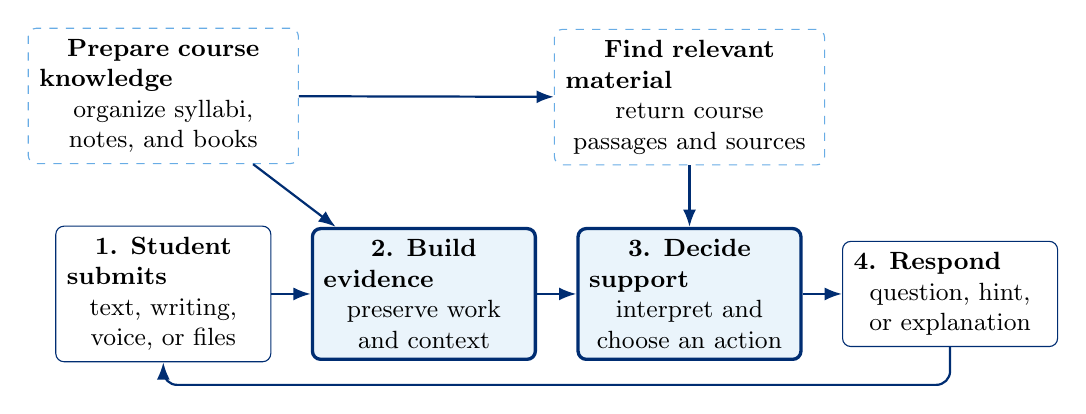
\begin{tikzpicture}[
  node distance=.60cm and .50cm,
  box/.style={draw=HopkinsBlue,rounded corners=3pt,fill=white,align=center,text width=2.45cm,minimum height=1.0cm,inner sep=4pt,font=\small},
  central/.style={draw=HopkinsBlue,very thick,rounded corners=3pt,fill=PaleBlue,align=center,text width=2.55cm,minimum height=1.05cm,inner sep=4pt,font=\small},
  support/.style={draw=SpiritBlue,dashed,rounded corners=3pt,fill=white,align=center,text width=3.15cm,minimum height=.88cm,inner sep=4pt,font=\small},
  arrow/.style={-{Latex[length=2.2mm]},thick,draw=HopkinsBlue}]

\node[support] (course) {\textbf{Prepare course knowledge}\newline organize syllabi, notes, and books};
\node[box,below=.78cm of course] (student) {\textbf{1. Student submits}\newline text, writing, voice, or files};
\node[central,right=of student] (integrate) {\textbf{2. Build evidence}\newline preserve work and context};
\node[central,right=of integrate] (decision) {\textbf{3. Decide support}\newline interpret and choose an action};
\node[box,right=of decision] (delivery) {\textbf{4. Respond}\newline question, hint, or explanation};
\node[support,above=.78cm of decision] (knowledge) {\textbf{Find relevant material}\newline return course passages and sources};

\draw[arrow] (student)--(integrate);
\draw[arrow] (integrate)--(decision);
\draw[arrow] (decision)--(delivery);
\draw[arrow] (course)--(knowledge);
\draw[arrow] (knowledge)--(decision);
\draw[arrow] (course)--(integrate);
\draw[arrow,rounded corners=5pt] (delivery.south) -- ++(0,-.48) -| (student.south);
\end{tikzpicture}
\vspace{.4em}

\begin{minipage}{.91\textwidth}
\small
The cycle repeats: each student response becomes new evidence, so the system can reassess what help is appropriate instead of treating every message as an isolated question.
\end{minipage}
\end{frame}

% 4. Lightweight prototype
\begin{frame}{Prototype status: what works today}
\begin{columns}[T,onlytextwidth]
\column{.49\textwidth}
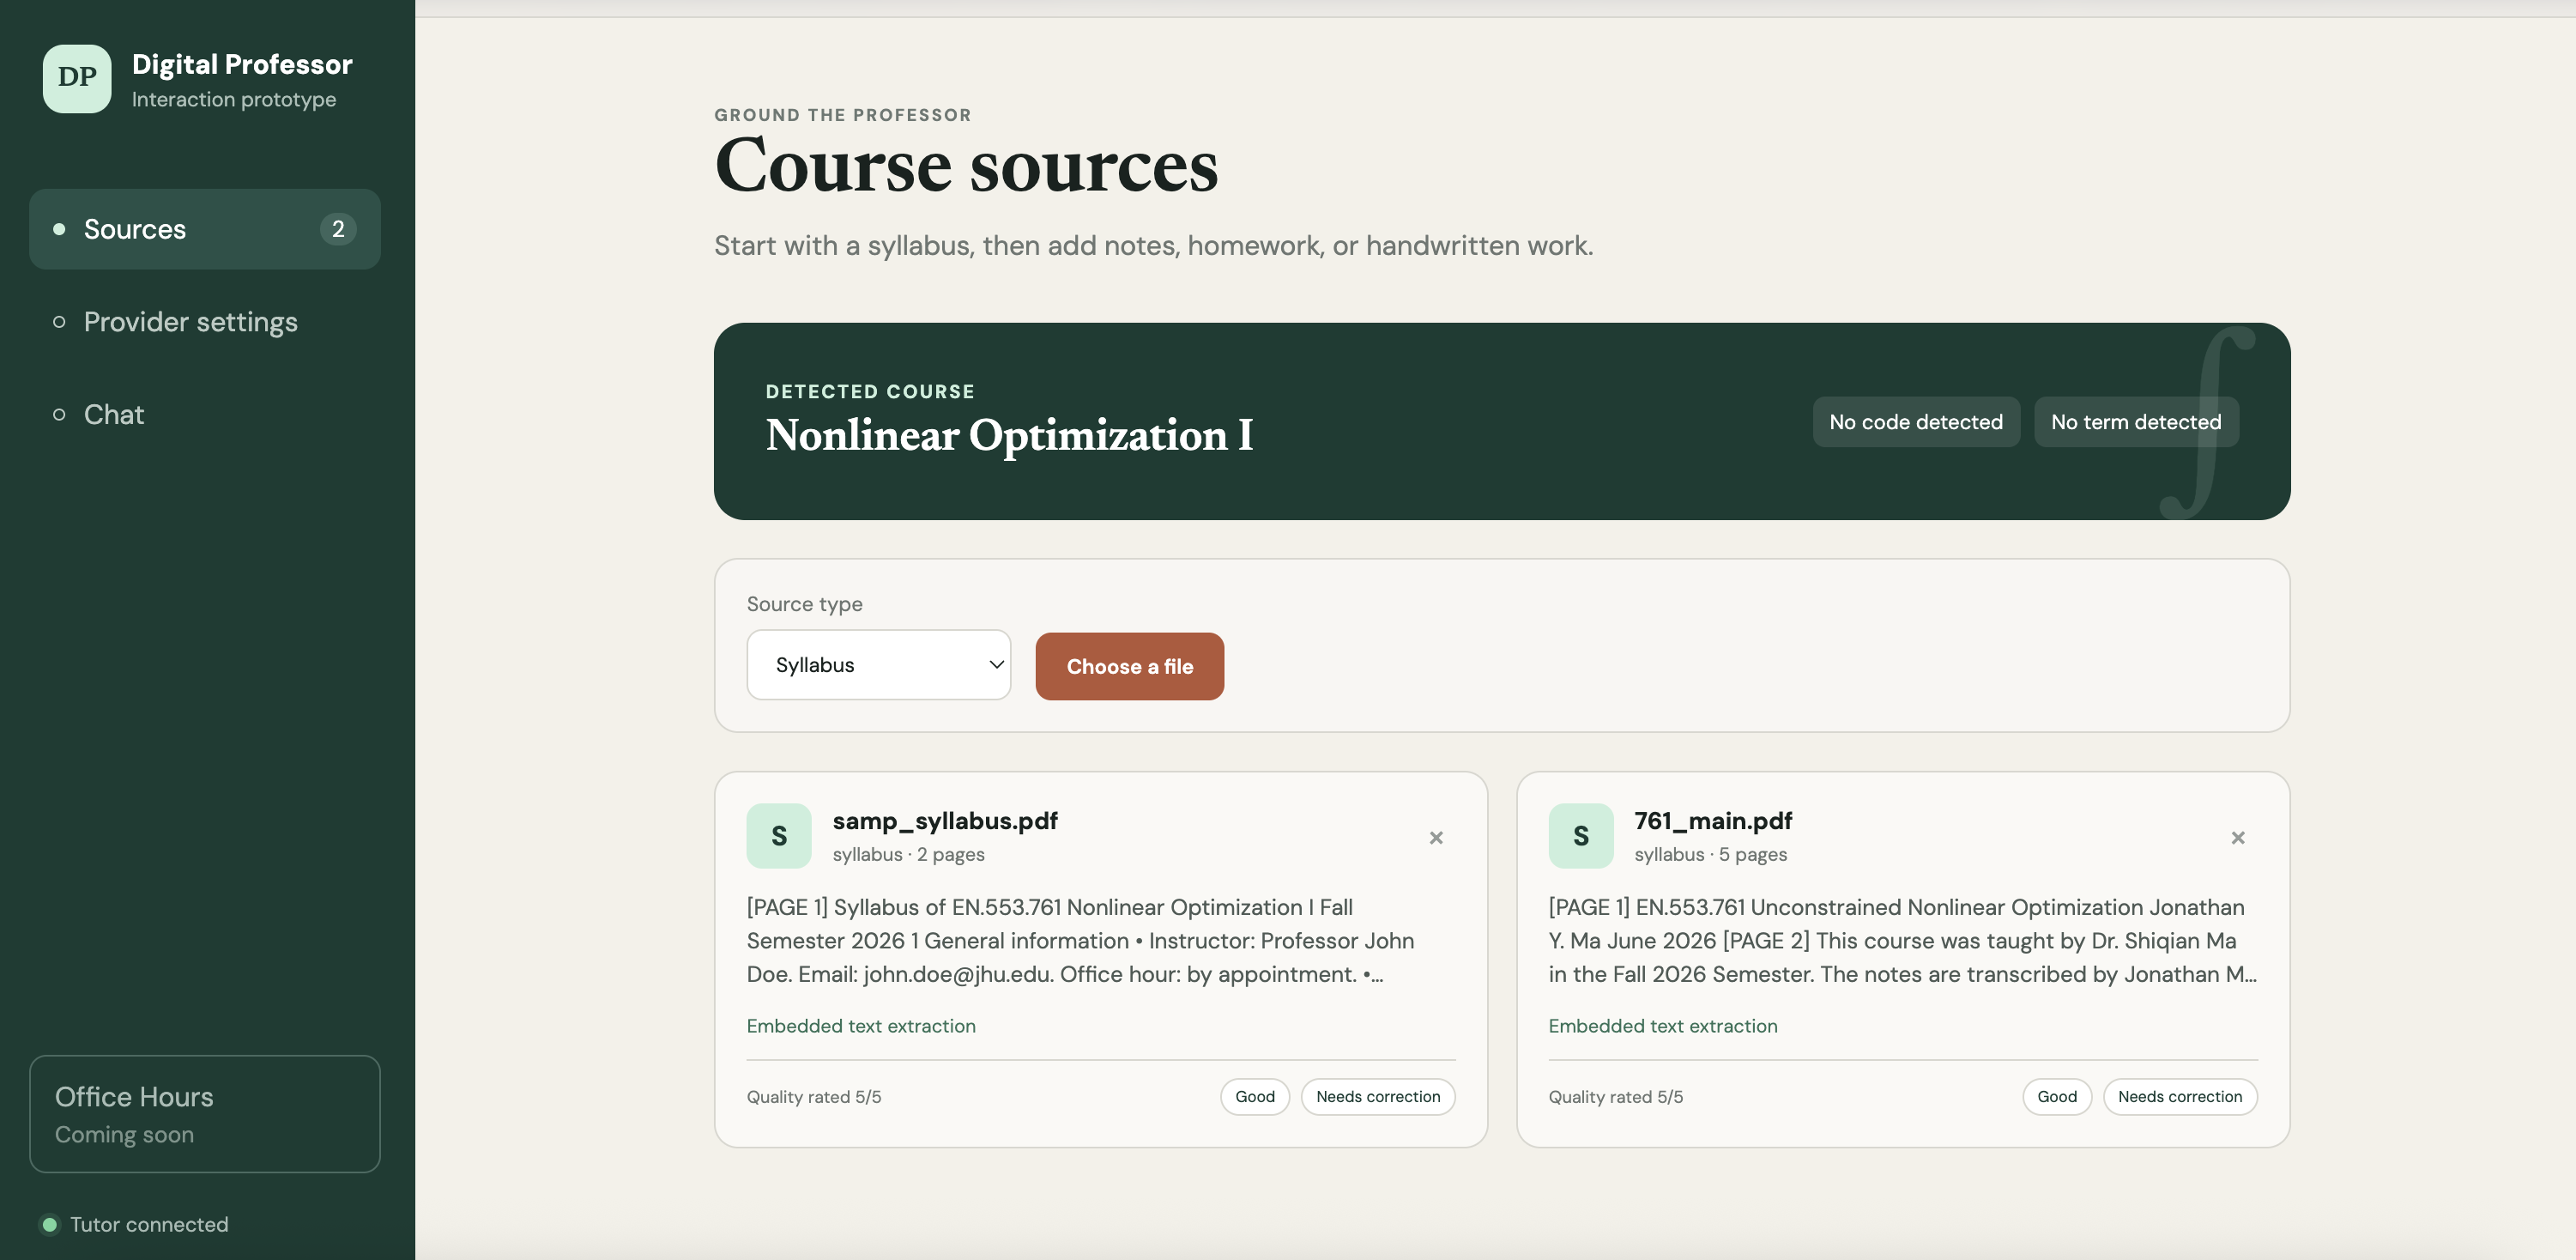
\includegraphics[width=\linewidth,height=.49\textheight,keepaspectratio]{landing_and_upload.png}
\vspace{.25em}

\begin{block}{Course material}
Upload documents, identify course information, preview extracted content, and flag uncertain results.
\end{block}
\column{.49\textwidth}
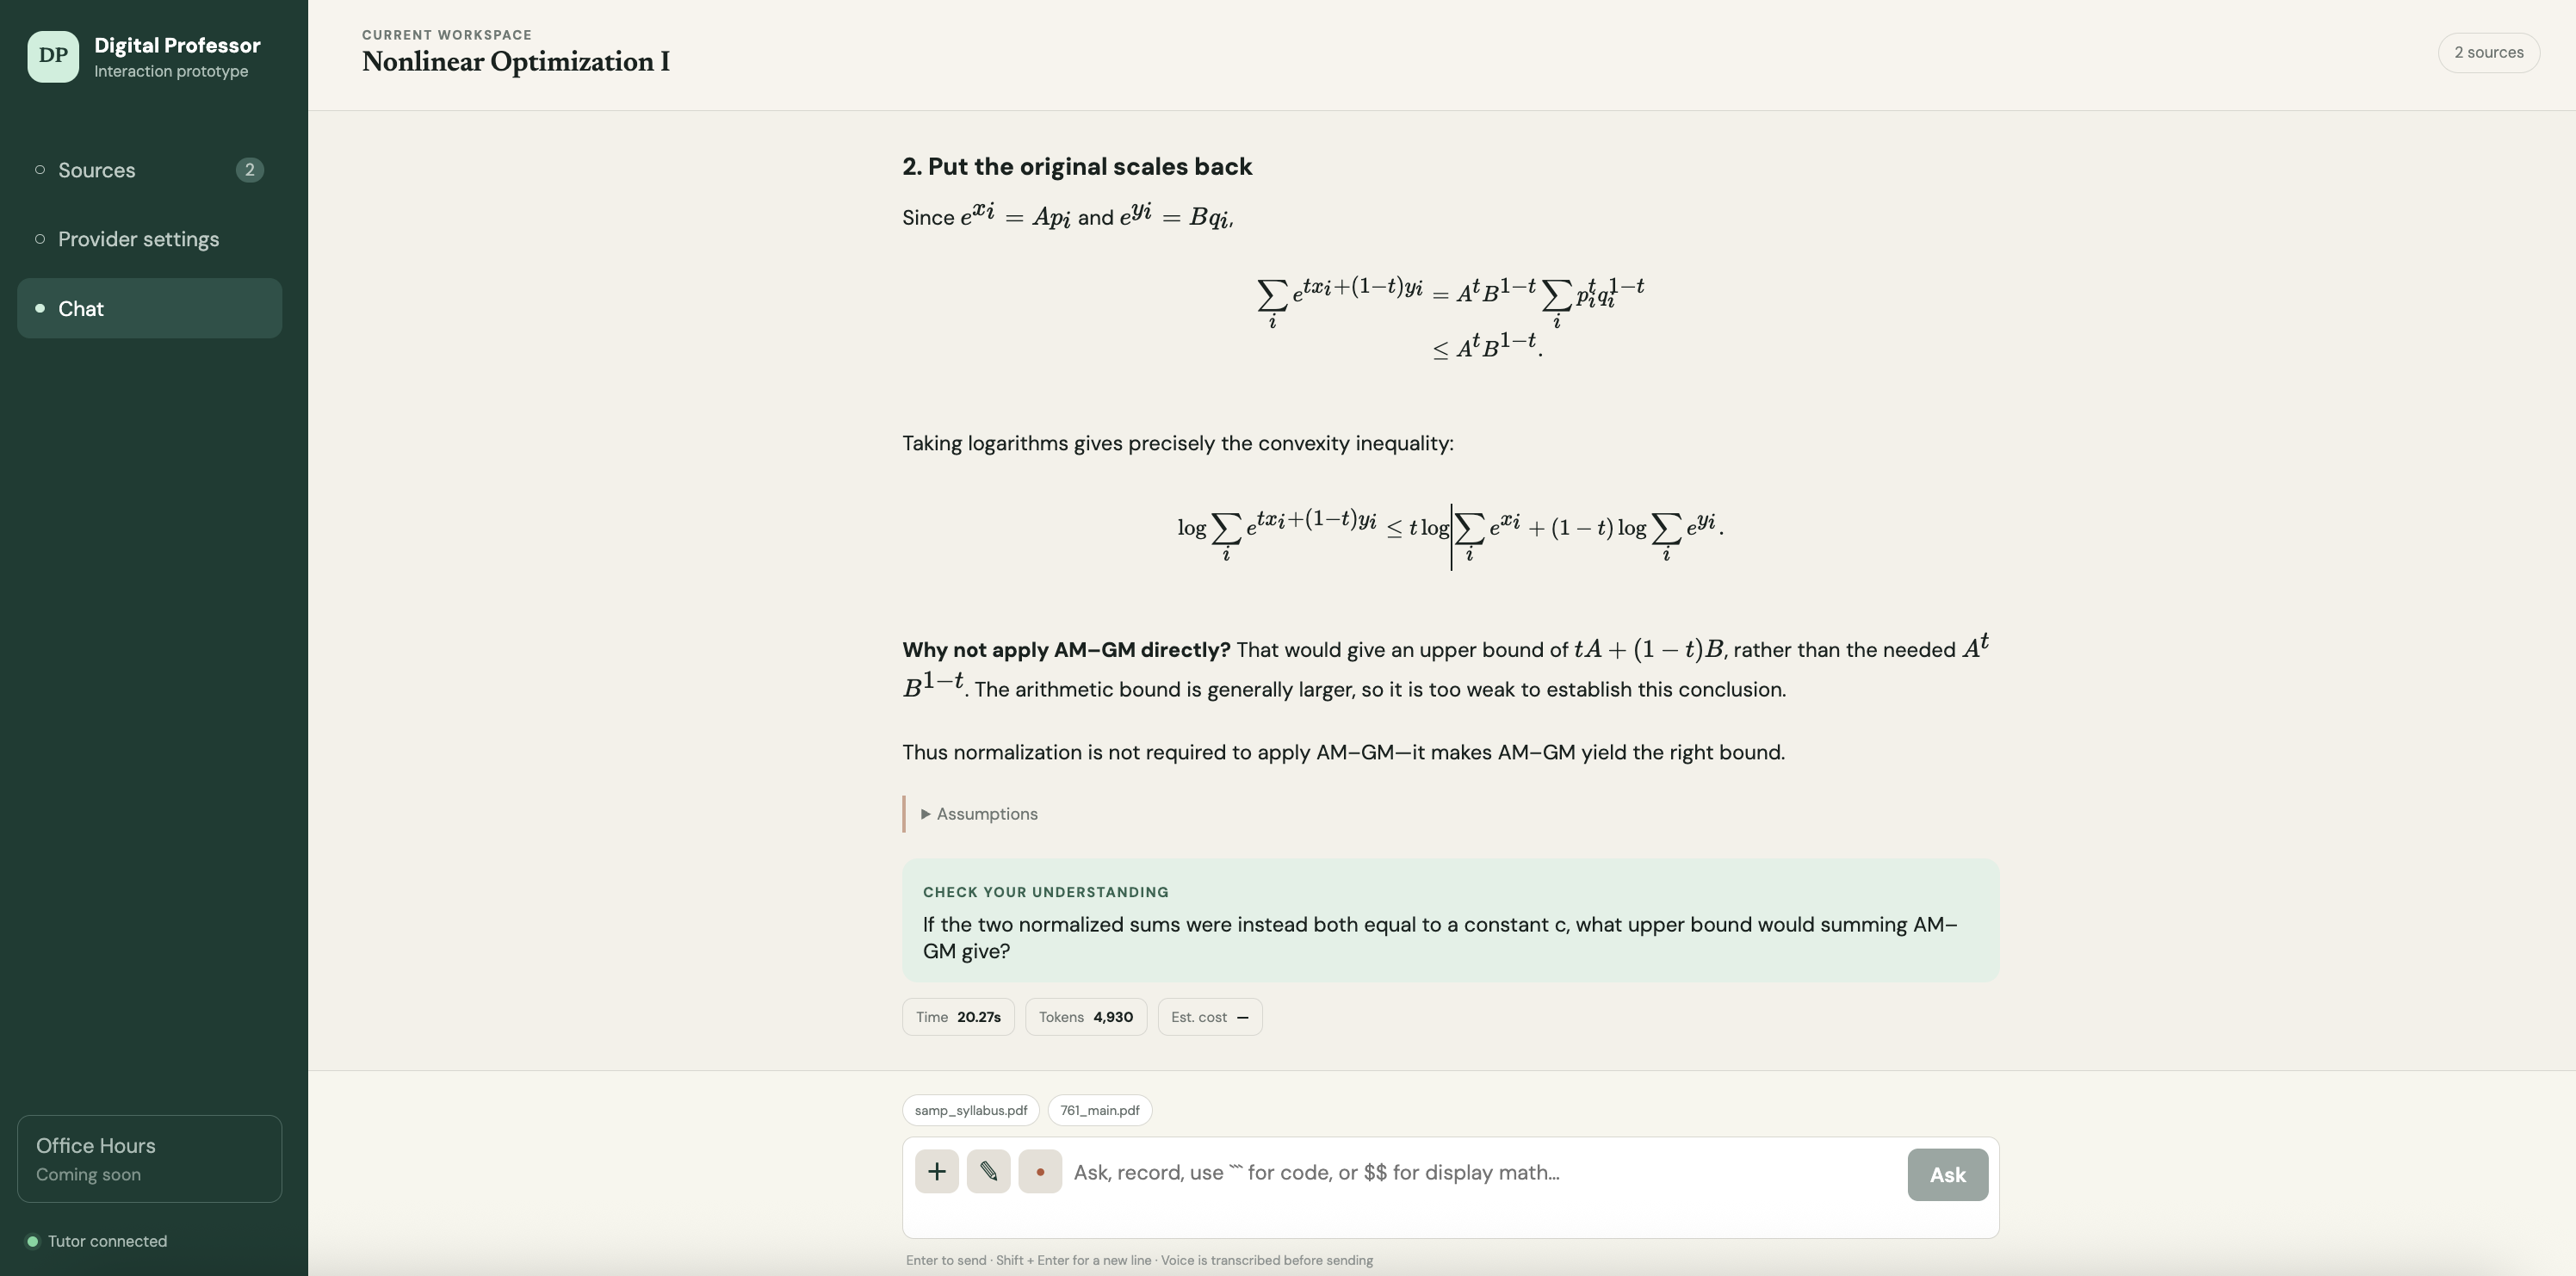
\includegraphics[width=\linewidth,height=.49\textheight,keepaspectratio]{chat_2.png}
\vspace{.25em}

\begin{block}{Student interaction}
Ask through text, equations, handwriting, or recorded voice; view rendered mathematics, cited sources, and request timing.
\end{block}
\end{columns}
\vspace{.2em}
\centering
\textbf{Current status:} a local research prototype demonstrates the main inputs and handoffs; it is not yet a complete adaptive tutor.
\end{frame}

% 5. Reserved for teammate content
\begin{frame}{Existing products}
\vspace{1em}
{\color{Muted}\itshape Compare relevant digital tutoring products in plain language: what students can do with them today, what they do well, and which gaps motivate our approach.}
\end{frame}

% 6. Reserved for Ovunc
\begin{frame}{Advanced course ingestion and context}
\vspace{1em}
{\color{Muted}\itshape Explain how syllabi, lecture notes, textbooks, and questions become reliable course context. Show what structured information is produced and how the tutoring system uses it.}
\end{frame}

% 7. Reserved for Sean
\begin{frame}{Course knowledge module: inputs, functions, and outputs}
\vspace{1em}
{\color{Muted}\itshape Sean should explain his module as one simple pipeline:}
\vspace{.8em}

\begin{columns}[T,onlytextwidth]
\column{.31\textwidth}
\begin{block}{Inputs}
List the course documents, structured course context, student question, and any filters the module receives.
\end{block}
\column{.31\textwidth}
\begin{block}{Functions}
Describe how material is divided, stored, searched, ranked, and checked for relevance.
\end{block}
\column{.34\textwidth}
\begin{block}{Outputs}
Show the passages, page references, confidence or status, and metadata returned to the tutoring system.
\end{block}
\end{columns}
\vspace{.55em}
\centering
{\color{Muted}\itshape Include one concrete example showing a question entering the module and the course evidence returned downstream.}
\end{frame}

% 8. Reserved for teammate content
\begin{frame}{Risk matrix}
\vspace{1em}
{\color{Muted}\itshape Show the few risks most likely to affect the project or student experience. Explain their impact and the practical step planned to reduce each one.}
\end{frame}

% 9. Goals for the second half
\begin{frame}{Future work}
\begin{columns}[T,onlytextwidth]
\column{.31\textwidth}
\begin{block}{1. Implement the architecture}
Connect course ingestion, knowledge retrieval, student evidence, tutoring decisions, and delivery through agreed interfaces.
\end{block}
\column{.31\textwidth}
\begin{block}{2. Build a Calculus test set}
Create representative course materials, student work, and tutoring situations covering correct, partial, incorrect, and uncertain responses.
\end{block}
\column{.34\textwidth}
\begin{block}{3. Review independently}
Have an independent mathematics reviewer verify mathematical correctness, use of course evidence, and the quality of tutoring decisions.
\end{block}
\end{columns}
\vspace{.7em}
\centering
\textbf{Second-half goal:} demonstrate a complete Calculus tutoring loop whose inputs, evidence, decisions, and feedback can all be inspected.
\end{frame}

% 10. Q&A
\begin{frame}[plain]
\vfill
\centering
{\color{HopkinsBlue}\Huge Questions?\par}
\vspace{.6em}
{\color{Muted}\large 5-minute Q\&A\par}
\vspace{1.2em}
{\color{SpiritBlue}\rule{2.3cm}{2pt}}\par
\vspace{1em}
{\small Ovunc Eker \quad Jonathan Ma \quad Sean Song \quad Yining Li}
\vfill
\end{frame}

\end{document}
